\section{Alternative Estimator Comparisons}
\label{app:alternative-estimators}

Because biometric registration rolls out at different times across municipalities, the main Callaway--Sant'Anna event studies are one way to summarize the dynamics under staggered adoption \citep{Callaway2020DifferenDifferenWith}. This appendix compares those main plots to dynamic TWFE, Borusyak--Jaravel--Spiess, and de Chaisemartin--D'Haultfoeuille alternatives \citep{Borusyak2024RevisitiEventStudy,deChaisemartin2020TwoWayFixed}. Across outcomes, the broad pattern is stable: BVR produces an immediate contraction in the registry and a persistent shift away from lower-education registrants and toward higher-education registrants. The main difference across estimators is precision at the longest horizons, where support becomes thin.

\begin{figure}[p]
    \caption{Biometric Registration and Electorate Size: Alternative Estimators}
    \label{fig:appendix-size-estimator-comparison}
    \centering
    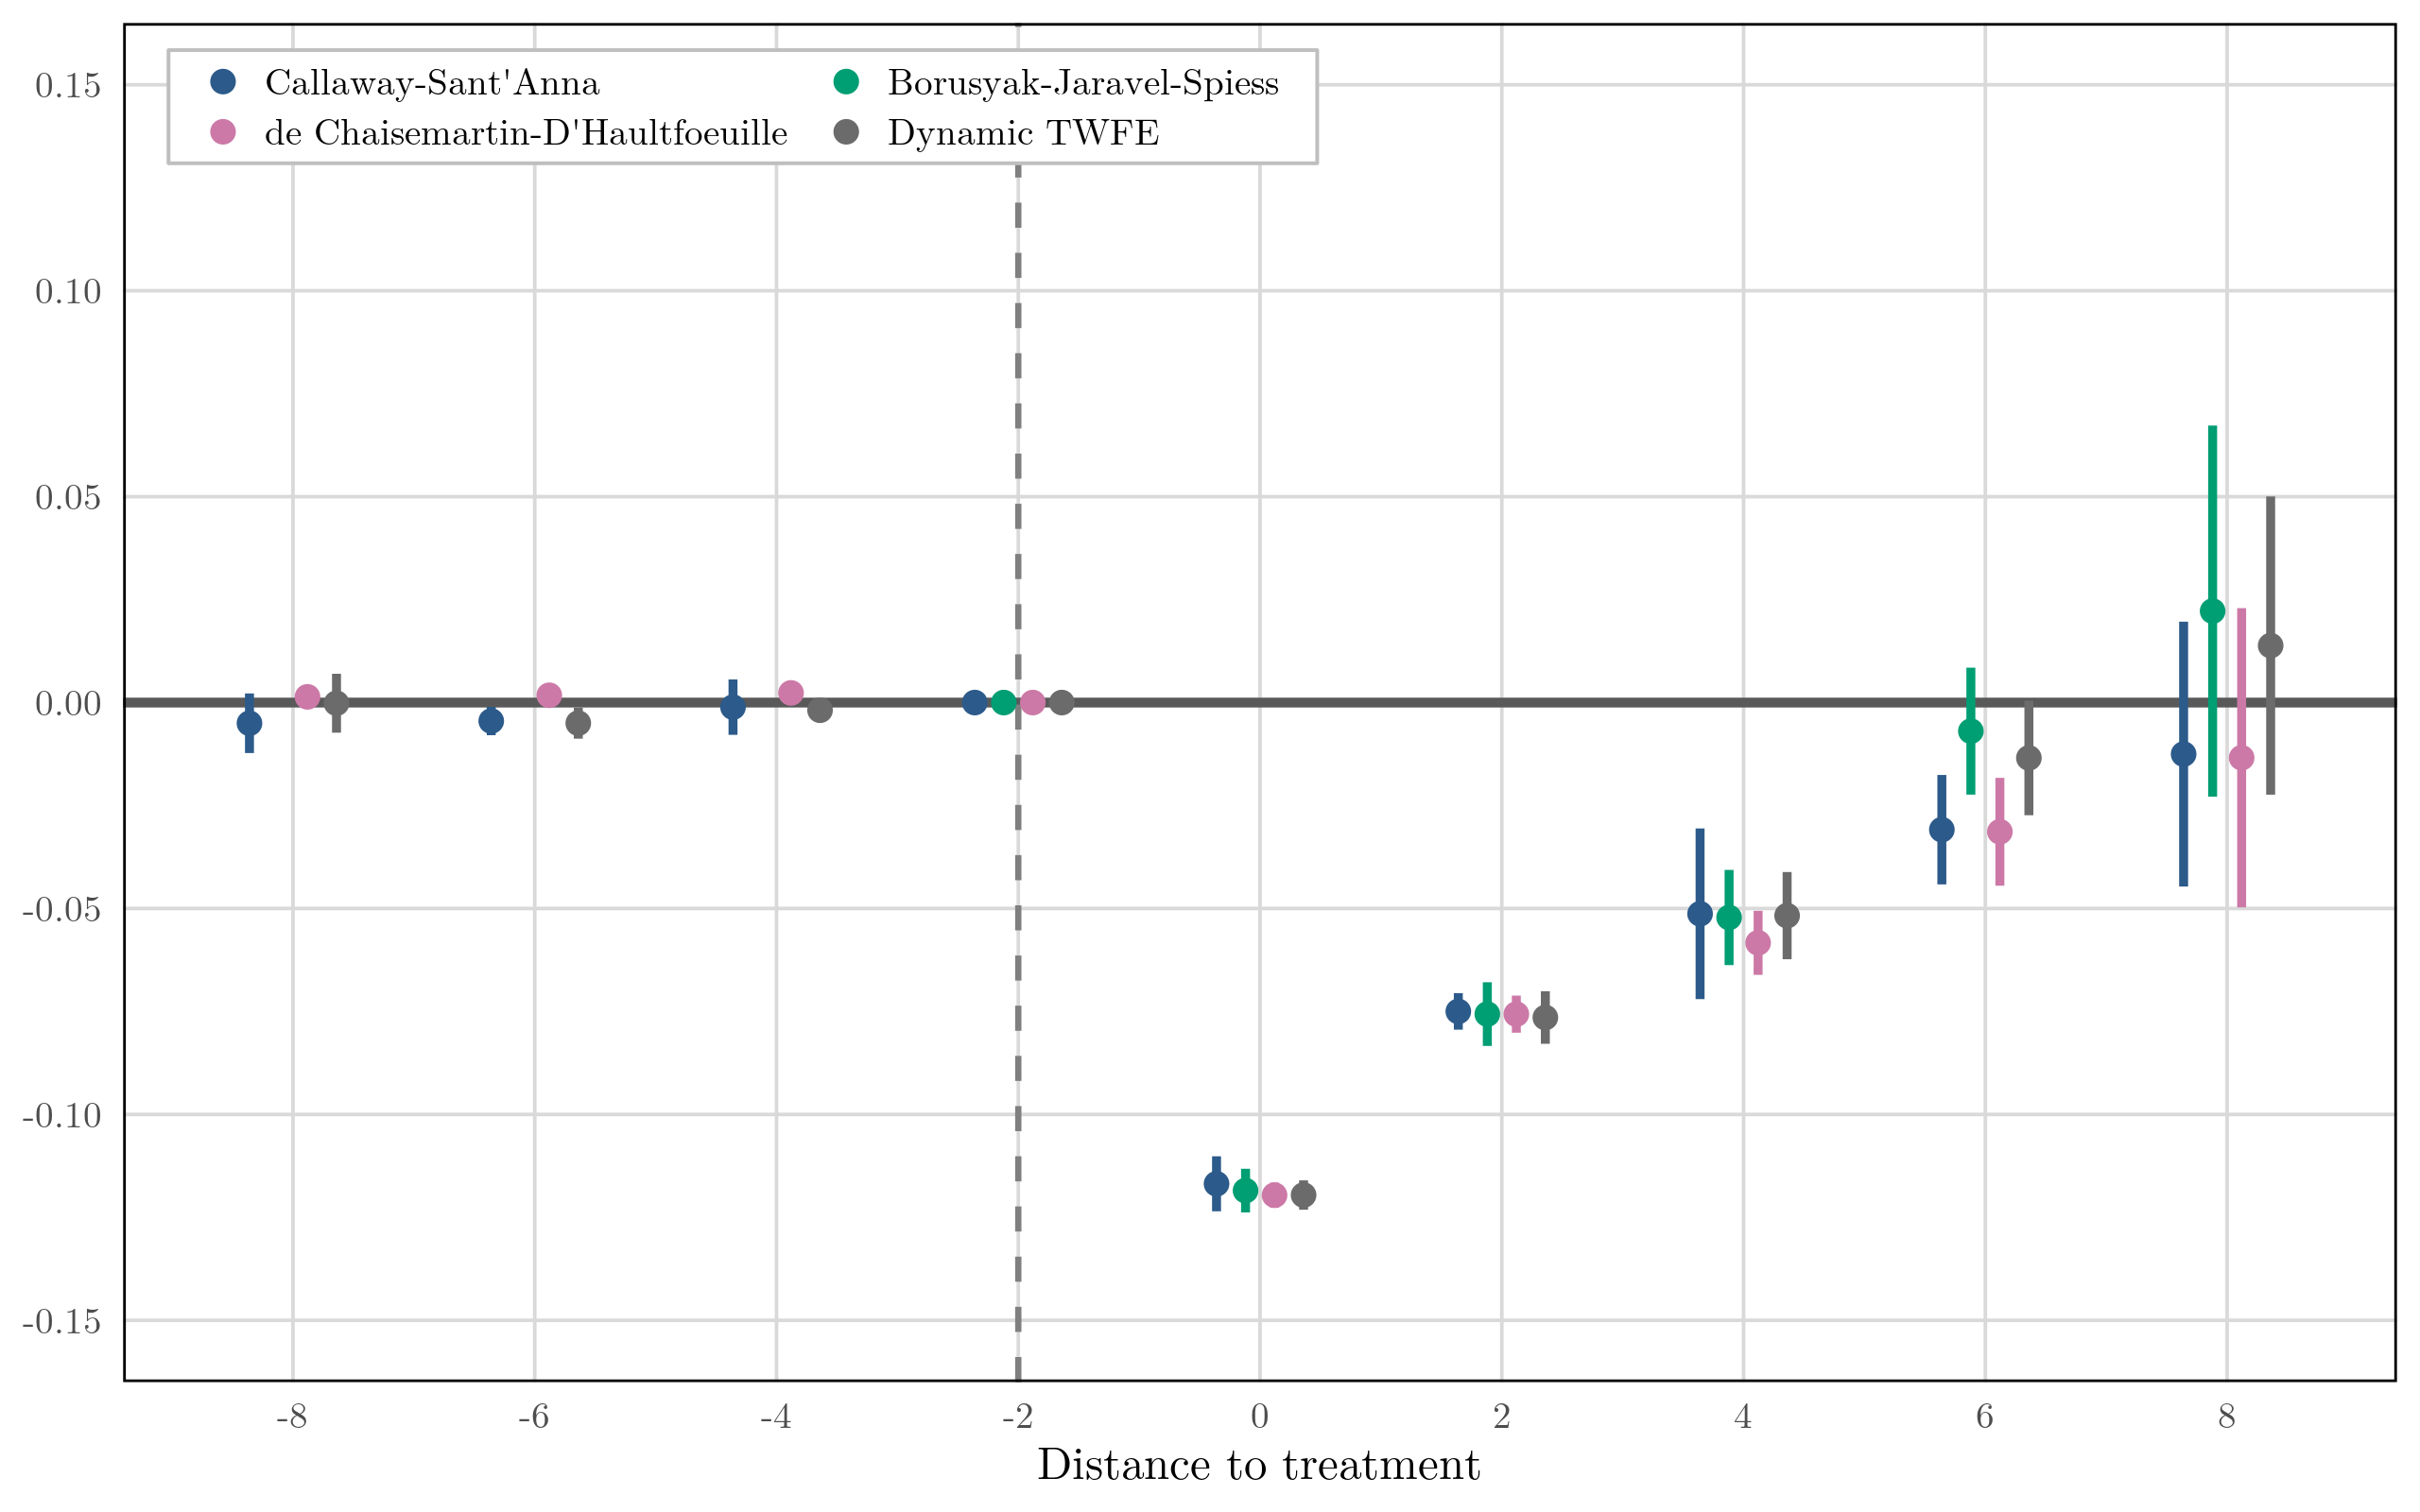
\includegraphics[width=0.72\textwidth]{../resources/regressions/bvr/log_num_voters/strict_bvr/other_estimators/estimator_comparison.png}
    \vspace{0.75em}
    \begin{minipage}{\textwidth}
        {\footnotesize \textbf{Note:} Each point reports an event-time estimate and each whisker a 95\% confidence interval. Colors identify the estimator. The Callaway--Sant'Anna series corresponds to the main event study in the text. The comparison series report dynamic TWFE, Borusyak--Jaravel--Spiess, and de Chaisemartin--D'Haultfoeuille estimators, using the same strict-BVR sample where available. \par}
    \end{minipage}
\end{figure}

\begin{figure}[p]
    \caption{Biometric Registration and Education Composition: Alternative Estimators}
    \label{fig:appendix-composition-estimator-comparison}
    \centering
    \begin{subfigure}[b]{0.49\textwidth}
        \centering
        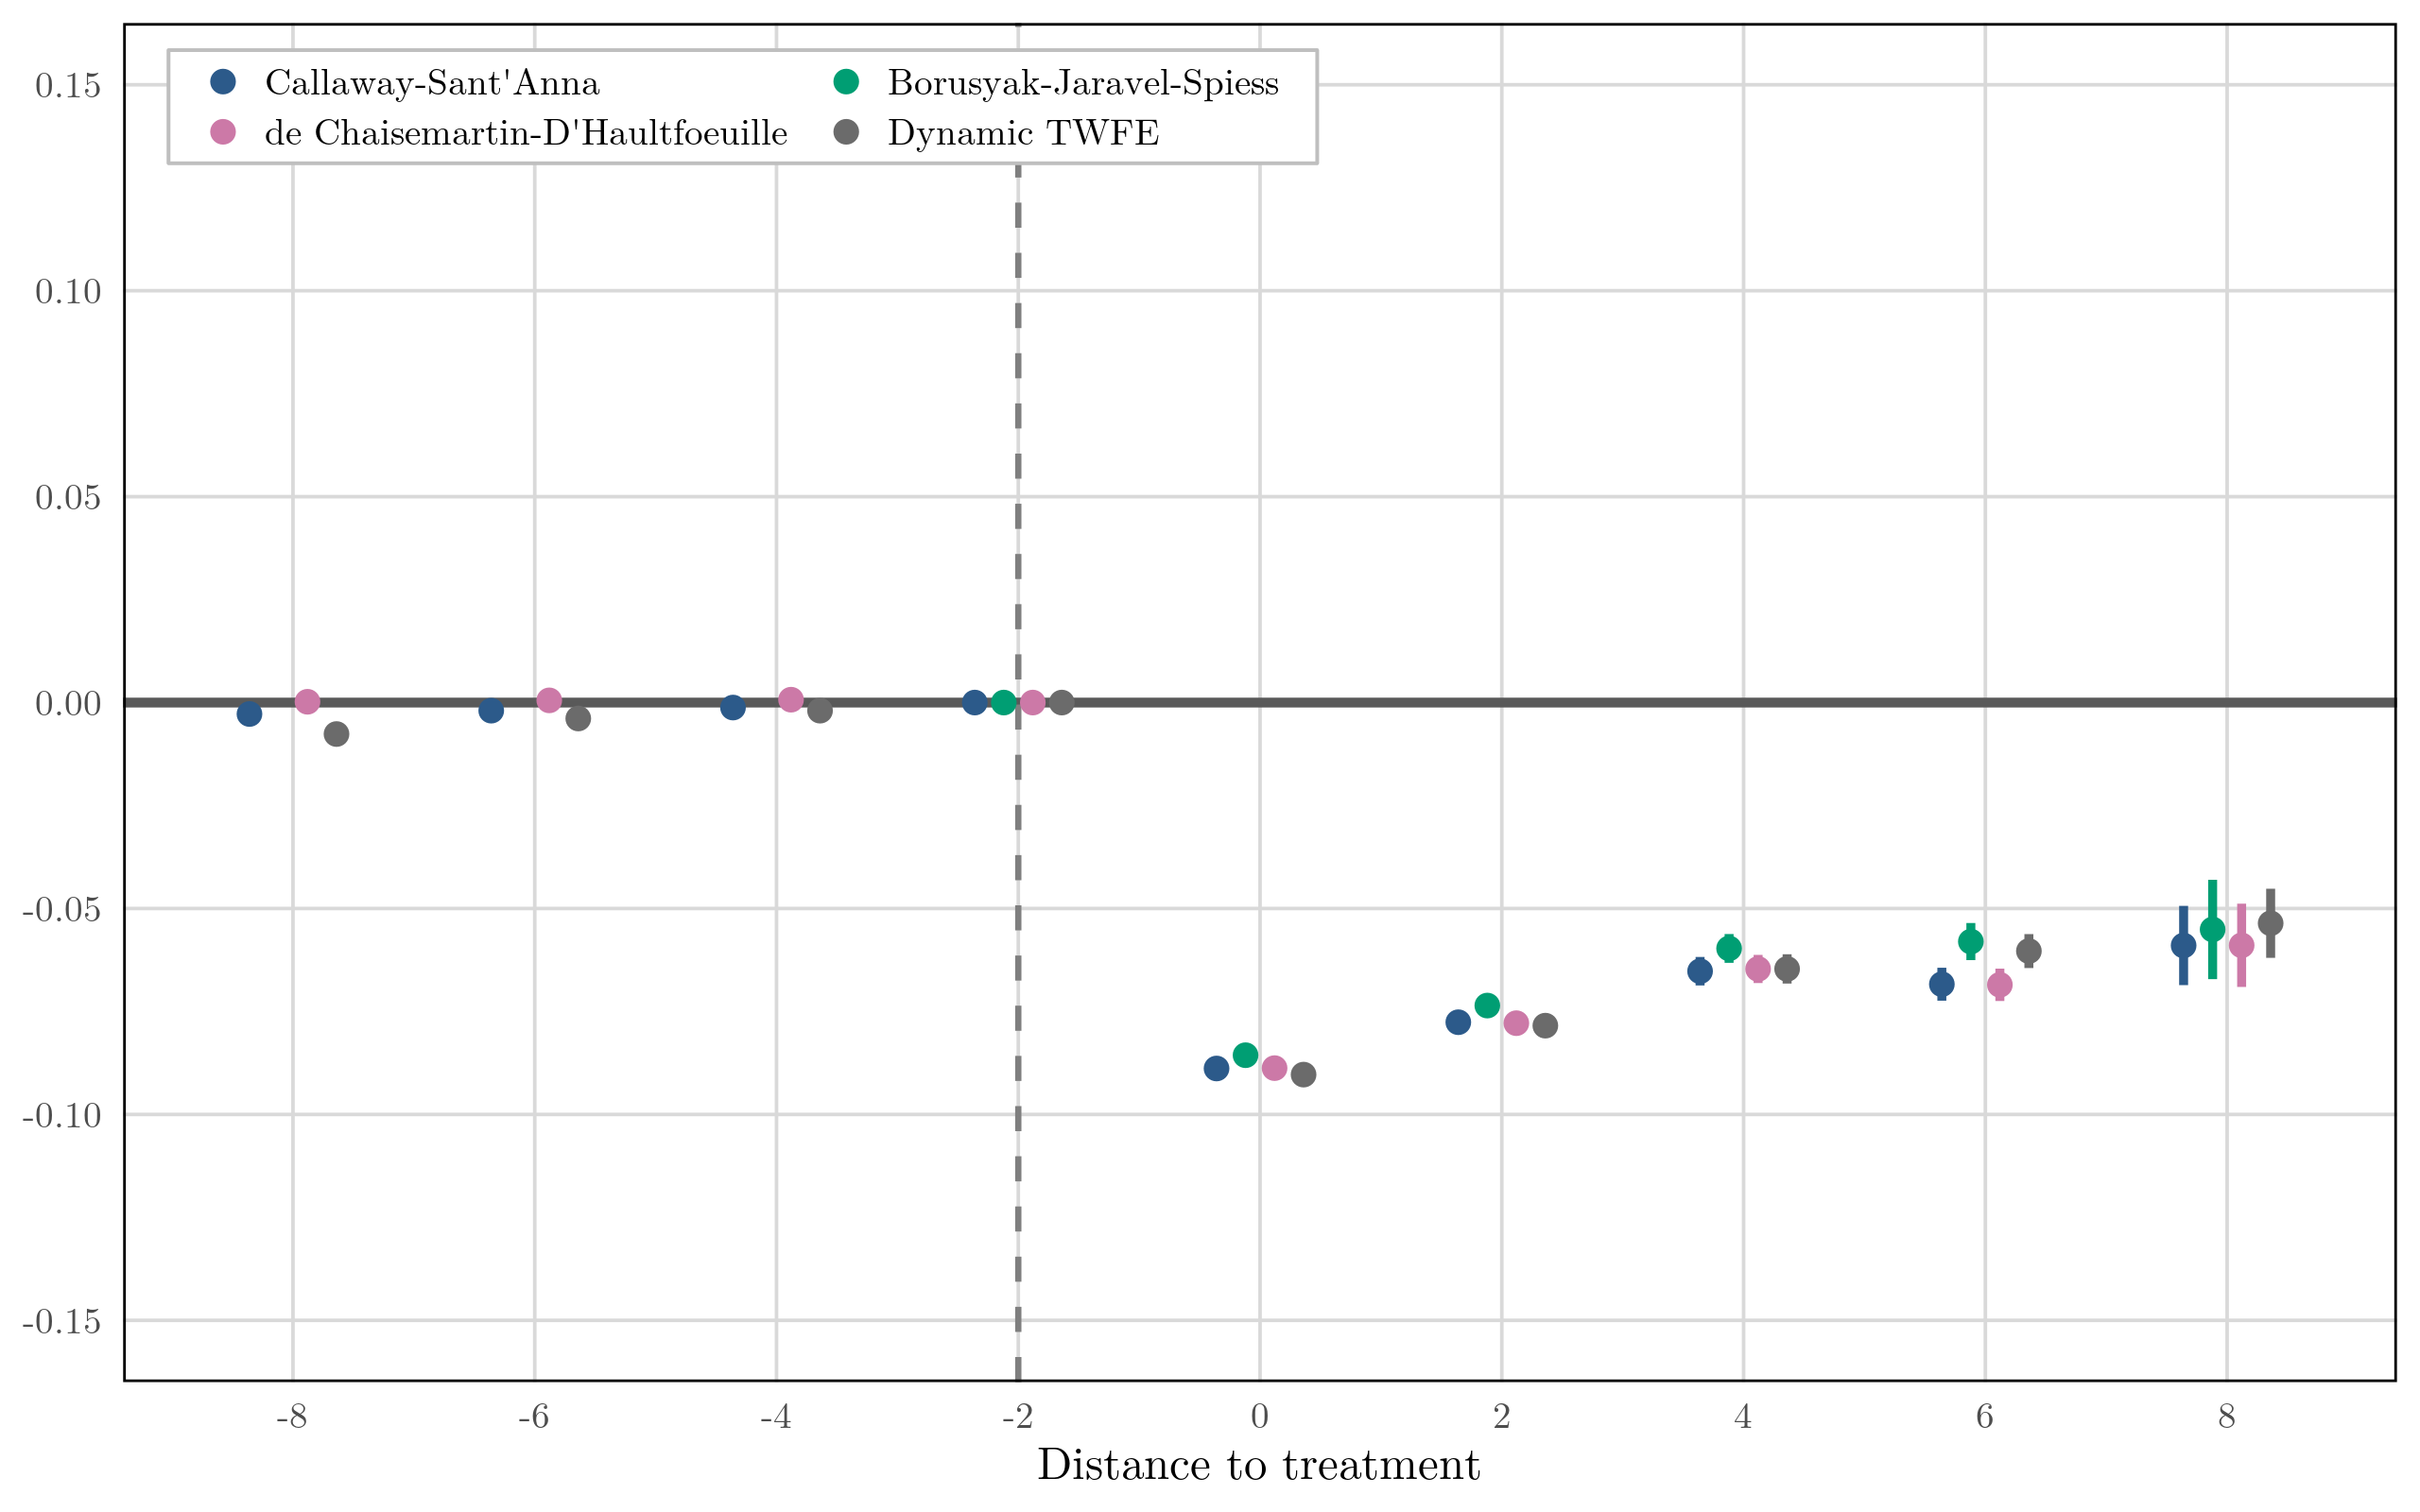
\includegraphics[width=\textwidth]{../resources/regressions/bvr/pct_voters_low_ed/strict_bvr/other_estimators/estimator_comparison.png}
        \caption{Low-education share}
        \label{fig:appendix-low-education-estimator-comparison}
    \end{subfigure}
    \hfill
    \begin{subfigure}[b]{0.49\textwidth}
        \centering
        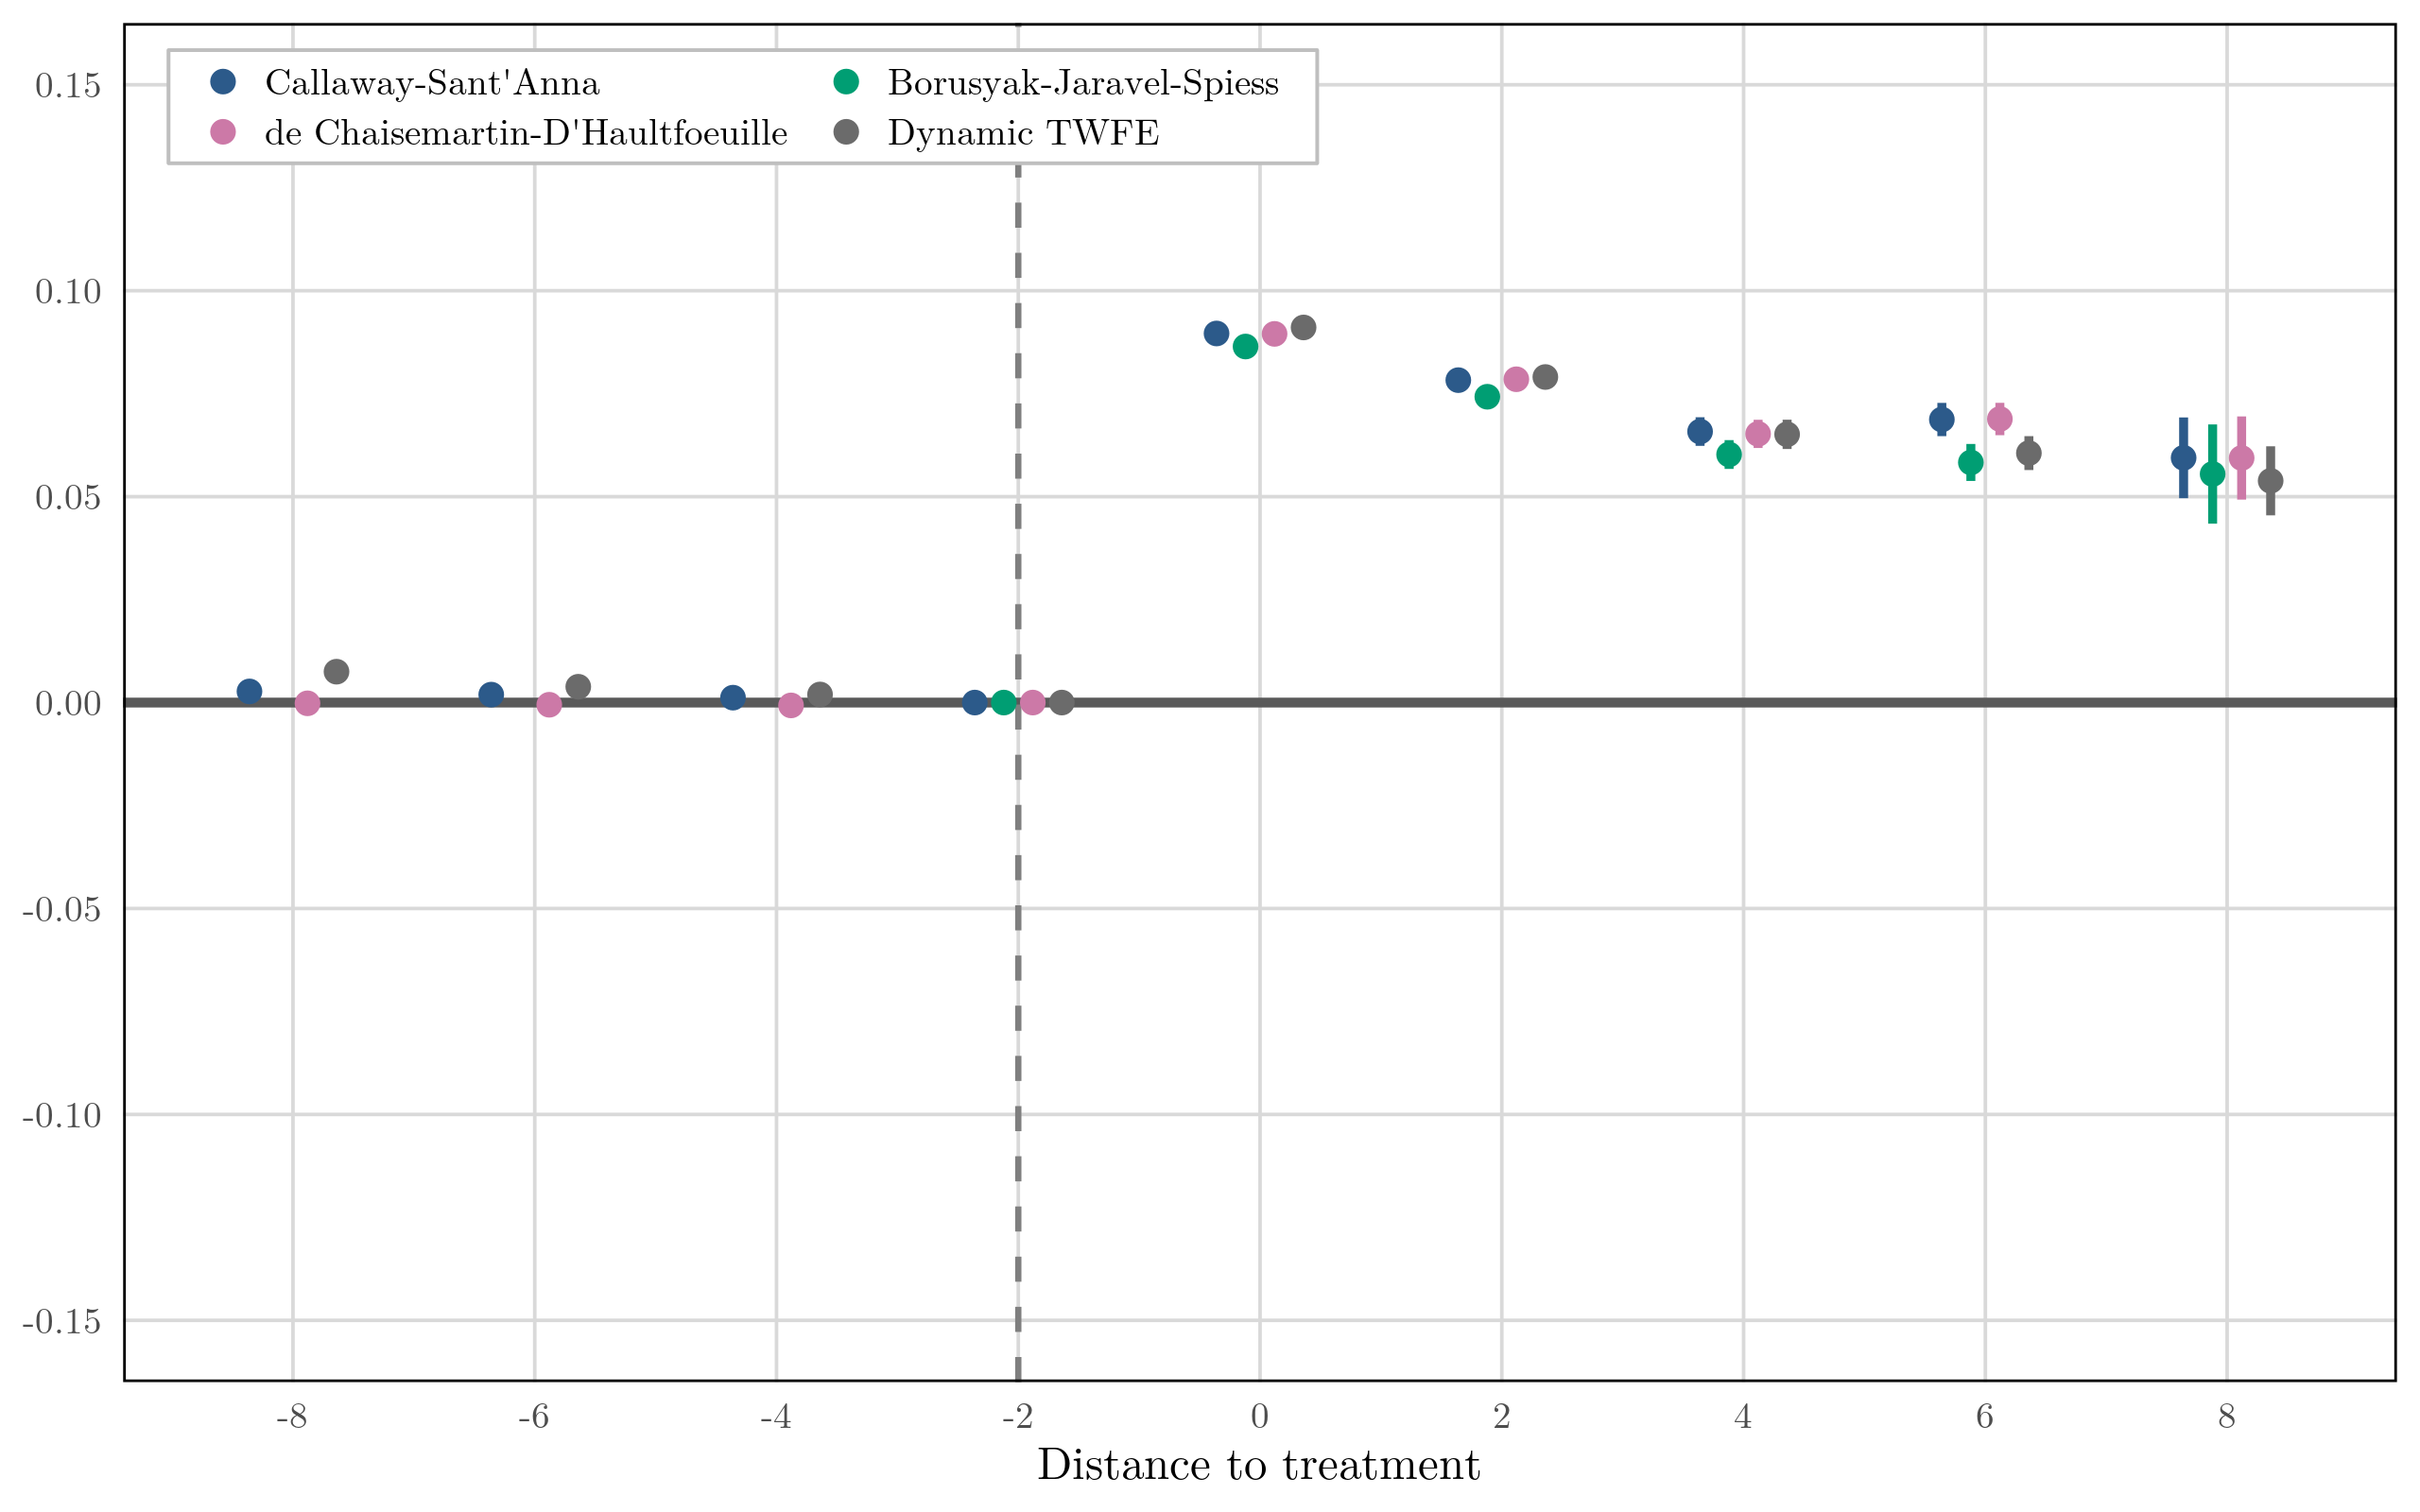
\includegraphics[width=\textwidth]{../resources/regressions/bvr/pct_voters_high_ed/strict_bvr/other_estimators/estimator_comparison.png}
        \caption{High-education share}
        \label{fig:appendix-high-education-estimator-comparison}
    \end{subfigure}
    \vspace{0.75em}
    \begin{minipage}{\textwidth}
        {\footnotesize \textbf{Note:} Each point reports an event-time estimate and each whisker a 95\% confidence interval. Colors identify the estimator. Panel (a) uses the share of registered voters with schooling below completed secondary education as the outcome, and panel (b) uses the share with incomplete secondary schooling or more. Across Callaway--Sant'Anna, dynamic TWFE, Borusyak--Jaravel--Spiess, and de Chaisemartin--D'Haultfoeuille estimators, the low-education share falls around biometric adoption and the high-education share rises, with the largest differences appearing in the noisier long-run horizons. \par}
    \end{minipage}
\end{figure}
